%!TEX root = ../main.tex
\chapter{Justificación económica}\label{cap:justificacion-economica}

Con el fin de dimensionar el beneficio de tiempo que aporta la solución propuesta, se relevó en la base de datos de producción la cantidad de concesionarios facturados en una muestra de 11 días hábiles (6 días para Chile, 5 días para Perú), combinando días cercanos al cierre de mes y días de mitad de mes, con el objetivo de evitar sesgar la muestra hacia los picos de actividad de fin de mes.

A partir de una prueba concreta (la carga manual de 3 concesionarios demandó aproximadamente 10 minutos), se estableció una tasa de referencia de \textasciitilde3,3 minutos por concesionario, aplicable tanto a Chile como a Perú, dado que el procedimiento (acceso al home banking, consulta del saldo, búsqueda del concesionario en CR08/CR12 y modificación manual del saldo disponible) es equivalente en ambos países.

Aplicando esta tasa a la muestra relevada, se obtuvo un promedio diario de aproximadamente 23,4 minutos para Chile y 20,7 minutos para Perú. Dado que la muestra reveló actividad en la totalidad de los días hábiles relevados, se proyectó el cálculo sobre una base de 250 días hábiles anuales, resultando en una estimación de aproximadamente 97,5 horas anuales para Chile y 86,3 horas anuales para Perú, es decir, un total combinado de aproximadamente 184 horas anuales dedicadas exclusivamente a la carga manual de crédito disponible en las pantallas CR08 y CR12.

Cabe destacar que esta estimación es conservadora: para los concesionarios que operan tanto unidades livianas como pesadas, el proceso actual requiere una carga separada en las pantallas CR08 y CR12 respectivamente, ya que el sistema no cuenta hoy con un mecanismo que determine automáticamente esta distribución. La estimación presentada no desagrega este escenario por falta de datos históricos precisos al respecto, por lo que el tiempo real invertido podría ser mayor al aquí calculado.

\section{Análisis de impacto}

\subsection{Justificación institucional}

La situación actual del proceso de facturación de unidades financiadas presenta un fuerte componente manual y secuencial. Un analista notifica al usuario de cuentas a cobrar qué unidades deben facturarse, indicando cantidad y líneas de crédito disponibles; dicho usuario debe entonces acceder al home banking de la entidad bancaria correspondiente para verificar el crédito, cargar manualmente esa información en el sistema, y recién entonces proceder a facturar si no se detectan errores. Una vez facturada la unidad, SAI notifica la legalidad correspondiente, pero el usuario no cuenta con visibilidad sobre el avance del proceso: debe revisar reiteradamente el estado de las unidades en VH Legacy hasta confirmar que la totalidad del lote fue facturado correctamente.

La situación deseada elimina la dependencia de la verificación manual del crédito disponible, automatizando la consulta y actualización directamente contra las entidades bancarias, y automatiza asimismo el reporte de las facturas emitidas. Adicionalmente, se incorpora una notificación automática por correo electrónico una vez que la totalidad de las unidades de un lote ha sido facturada exitosamente, eliminando la necesidad de que el usuario revise manualmente el estado del proceso. En conjunto, estos cambios reducen el tiempo operativo dedicado a tareas repetitivas y disminuyen la probabilidad de errores humanos derivados de la carga manual de datos.

\subsection{Justificación legal}

No se identifica una normativa o regulación legal que exija específicamente la implementación de esta solución. La motivación del proyecto es de carácter operativo, orientada a reducir el tiempo dedicado a tareas manuales y a disminuir los errores humanos asociados al proceso actual de facturación.

\subsection{Justificación ambiental}

No aplica. La solución no genera un impacto ambiental significativo, dado que se trata de una automatización de procesos administrativos internos que no involucra cambios en el uso de recursos físicos o energéticos más allá de los propios de la operación habitual de los sistemas informáticos de la organización.

\subsection{Justificación social}

El concesionario depende directamente de que las unidades financiadas se facturen a tiempo, ya que de ello depende su propia operatoria comercial. Cualquier demora en el proceso actual repercute de forma encadenada sobre el concesionario: si el analista demora en enviar la información de las unidades a facturar, esa demora se traslada a la carga de datos por parte del usuario de cuentas a cobrar, lo cual retrasa a su vez la facturación y, finalmente, el envío de la información a la entidad bancaria. Al reducir los tiempos manuales y automatizar la comunicación con los bancos, la solución propuesta acorta esta cadena de demoras y contribuye a una facturación más ágil y predecible para el concesionario.

\section{Generación de archivo Excel para Santander}

Además del tiempo dedicado a la carga de crédito, el proceso actual de facturación hacia Perú requiere la generación manual de un archivo Excel por cada concesionario incluido en la facturación, con información particular de cada unidad (VIN, precio, DUA, entre otros datos), demandando cada archivo un tiempo superior a los 10 minutos.

\begin{figure}[H]
\centering
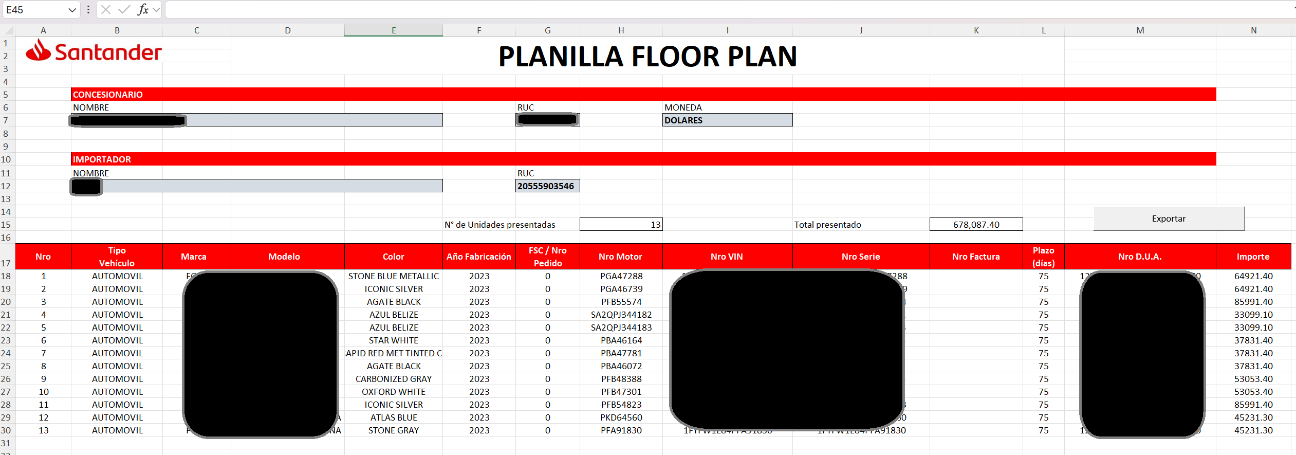
\includegraphics[width=1.00\textwidth]{figuras/image10}
\caption{Formato del archivo Excel de carga manual para Santander}\label{fig:9}
\end{figure}

Aplicando este tiempo de referencia (10 minutos, como valor conservador dado que el tiempo real reportado es superior) sobre la misma muestra de 5 días hábiles relevada para Perú (9, 4, 6, 5 y 7 concesionarios facturados respectivamente), se obtiene un promedio diario de 62 minutos, equivalente a aproximadamente \textbf{258 horas anuales} proyectadas sobre 250 días hábiles. Esta tarea es exclusiva de Perú. En Chile, el archivo que se enviaba a Forum por FTP era generado por el sistema, por lo que no requería armado manual; el usuario solo disparaba el envío desde una pantalla una vez verificada la facturación. Ese paso, junto con el tiempo que demandaba investigar los envíos fallidos revisando procesos del servidor y consultando a la entidad, no se incluye en la estimación por falta de datos que permitan cuantificarlo, por lo que el ahorro calculado para Chile es conservador.

En conjunto, el tiempo manual relevado para Perú ---carga de crédito (86,3 horas anuales) y generación de archivos para el banco (258 horas anuales)--- asciende a aproximadamente \textbf{344 horas anuales}, mientras que para Chile el tiempo relevado se limita a las 97,5 horas anuales de carga de crédito. El total combinado estimado para ambos países es de aproximadamente \textbf{442 horas anuales} dedicadas a tareas manuales que la solución propuesta automatiza.

\section{Evaluación económica}

Las secciones anteriores cuantificaron el beneficio del proyecto en horas de trabajo manual evitadas. Para completar el análisis, esta sección valoriza ese ahorro en términos monetarios, lo compara con el costo de desarrollo de la solución y calcula el valor actual neto (VAN) y el período de repago bajo dos horizontes de evaluación.

La inversión del proyecto se compone exclusivamente de horas de trabajo. El desarrollo y las pruebas demandaron aproximadamente 220 horas del autor entre mediados de agosto y mediados de octubre de 2026, equivalentes a unas 24 horas semanales durante nueve semanas. No se incurrió en costos de licencias, infraestructura ni servicios adicionales, ya que la solución se implementó sobre plataformas que la organización ya utilizaba, como Oracle, OpenShift y Google Cloud Platform. Tampoco se imputan al proyecto la configuración de Apigee, realizada por el equipo de DevOps como parte de una iniciativa organizacional que el proyecto adoptó con cambios menores, ni las herramientas de software que el autor ya utilizaba por otros motivos, por tratarse de costos no incrementales.

Para valorizar las horas se adoptó un costo de mercado tanto para el perfil de desarrollo como para el de análisis contable. En ambos casos se tomó como referencia un salario bruto mensual de \$2.500.000, es decir, previo a cargas sociales e impuestos: para el desarrollador, la mediana correspondiente al nivel semi senior en desarrollo de software según la encuesta de sueldos 2026.01 de SysArmy \citep{openqube2026}, cuyos resultados también fueron analizados por el \citet{dcuba2026}; para el analista contable, el rango observado en ofertas laborales publicadas en el portal Bumeran en octubre de 2026. Considerando trece salarios anuales, que incluyen el sueldo anual complementario, y una dedicación de 160 horas mensuales, el costo resultante es de aproximadamente \$16.927 por hora. Para expresar los valores en una moneda estable, se convirtieron a dólares estadounidenses al tipo de cambio mayorista de octubre de 2026, de aproximadamente \$1.530 por dólar, lo que arroja un costo de USD 11,06 por hora. No se incluyeron las contribuciones patronales: al afectar en la misma proporción a la inversión y al ahorro, su exclusión no modifica el período de repago y reduce el VAN, por lo que constituye un criterio conservador.

Con estos valores, la inversión inicial asciende a USD 2.434 y el ahorro de 442 horas anuales equivale a USD 4.890 por año. A este ahorro se le descuenta un costo de mantenimiento estimado en el 10 \% anual de la inversión, destinado a soporte y ajustes, de modo que el flujo neto resultante es de aproximadamente USD 387 por mes.

Como tasa de descuento se utilizó el costo promedio ponderado del capital (WACC) de la industria automotriz, de 9,38 \% anual en dólares según la base de datos de \citet{damodaran2026}, que representa la rentabilidad mínima que el mercado exige a las empresas del sector. Los flujos se descontaron en forma mensual, con la tasa equivalente de 0,75 \% mensual. La Tabla~\ref{tab:2} resume los supuestos utilizados.

\begin{longtable}[]{@{}
  >{\raggedright\arraybackslash}p{(\columnwidth - 4\tabcolsep) * \real{0.3334}}
  >{\raggedright\arraybackslash}p{(\columnwidth - 4\tabcolsep) * \real{0.3333}}
  >{\raggedright\arraybackslash}p{(\columnwidth - 4\tabcolsep) * \real{0.3334}}@{}}
\caption{Supuestos de la evaluación económica}\label{tab:2}\\
\toprule\noalign{}
\begin{minipage}[b]{\linewidth}\raggedright
Supuesto
\end{minipage} & \begin{minipage}[b]{\linewidth}\raggedright
Valor
\end{minipage} & \begin{minipage}[b]{\linewidth}\raggedright
Fuente o criterio
\end{minipage} \\
\midrule\noalign{}
\endfirsthead
\caption[]{Supuestos de la evaluación económica (continuación)}\\
\toprule\noalign{}
\begin{minipage}[b]{\linewidth}\raggedright
Supuesto
\end{minipage} & \begin{minipage}[b]{\linewidth}\raggedright
Valor
\end{minipage} & \begin{minipage}[b]{\linewidth}\raggedright
Fuente o criterio
\end{minipage} \\
\midrule\noalign{}
\endhead
\bottomrule\noalign{}
\endlastfoot
Inversión & 220 horas & Horas de desarrollo y pruebas del autor \\
Ahorro anual & 442 horas & Estimación de este capítulo \\
Salario bruto mensual de referencia & \$2.500.000 & SysArmy \citep{openqube2026} y ofertas en \citet{bumeran2026} \\
Costo por hora & \$16.927 (USD 11,06) & 13 salarios anuales y 160 horas mensuales \\
Tipo de cambio & \$1.530 por dólar & Dólar mayorista, octubre de 2026 \\
Mantenimiento & 10 \% anual de la inversión & Supuesto del autor \\
Tasa de descuento & 9,38 \% anual (0,75 \% mensual) & WACC de la industria automotriz \citep{damodaran2026} \\
\end{longtable}

Se evaluaron dos horizontes. El escenario conservador limita el análisis a 14 meses, entre noviembre de 2026 y diciembre de 2027, fecha prevista para la baja de VH, y supone que el beneficio se pierde a partir de ese momento. El escenario base extiende el horizonte a tres años, considerando que la funcionalidad de integración bancaria se migrará a otra aplicación de la empresa y que el ahorro operativo continuará. El costo de esa migración no se imputa al proyecto, dado que responde a la baja de VH y se realizaría con independencia de esta solución. La Tabla~\ref{tab:3} presenta los resultados de ambos escenarios.

\begin{longtable}[]{@{}
  >{\raggedright\arraybackslash}p{(\columnwidth - 4\tabcolsep) * \real{0.3334}}
  >{\raggedright\arraybackslash}p{(\columnwidth - 4\tabcolsep) * \real{0.3333}}
  >{\raggedright\arraybackslash}p{(\columnwidth - 4\tabcolsep) * \real{0.3334}}@{}}
\caption{Resultados de la evaluación económica por escenario}\label{tab:3}\\
\toprule\noalign{}
\begin{minipage}[b]{\linewidth}\raggedright
Indicador
\end{minipage} & \begin{minipage}[b]{\linewidth}\raggedright
Conservador (14 meses)
\end{minipage} & \begin{minipage}[b]{\linewidth}\raggedright
Base (3 años)
\end{minipage} \\
\midrule\noalign{}
\endfirsthead
\caption[]{Resultados de la evaluación económica por escenario (continuación)}\\
\toprule\noalign{}
\begin{minipage}[b]{\linewidth}\raggedright
Indicador
\end{minipage} & \begin{minipage}[b]{\linewidth}\raggedright
Conservador (14 meses)
\end{minipage} & \begin{minipage}[b]{\linewidth}\raggedright
Base (3 años)
\end{minipage} \\
\midrule\noalign{}
\endhead
\bottomrule\noalign{}
\endlastfoot
Inversión inicial & USD 2.434 & USD 2.434 \\
Ahorro anual & USD 4.890 & USD 4.890 \\
Mantenimiento anual & USD 243 & USD 243 \\
Flujo neto mensual & USD 387 & USD 387 \\
Valor actual neto (VAN) & USD 2.694 & USD 9.743 \\
Período de repago simple & 6,3 meses & 6,3 meses \\
Período de repago descontado & 7 meses & 7 meses \\
\end{longtable}

En ambos escenarios el VAN es positivo y la inversión se recupera en aproximadamente siete meses, hacia mayo de 2027, antes de la baja prevista de VH. En términos concretos, un VAN de USD 2.694 significa que, aun en el escenario más restrictivo, el proyecto recupera la inversión, cubre la rentabilidad mínima exigida al sector y genera además un valor adicional equivalente a unos USD 2.700.

Dado que los costos por hora y la tasa de descuento son supuestos, se analizó la sensibilidad del resultado frente a un costo del desarrollador un 30 \% superior y a tasas de descuento del 15 \% y del 25 \% anual, que incorporan el riesgo de operar en la región. Como muestra la Tabla~\ref{tab:4}, en el caso más desfavorable el VAN se mantiene positivo y el repago no supera los nueve meses. Se observa además que el período de repago depende de la relación entre el costo por hora del desarrollador y el del analista más que de sus valores absolutos: mientras el primero no supere el doble del segundo, la inversión se recupera dentro del horizonte conservador de 14 meses.

\begin{longtable}[]{@{}
  >{\raggedright\arraybackslash}p{(\columnwidth - 6\tabcolsep) * \real{0.2517}}
  >{\raggedright\arraybackslash}p{(\columnwidth - 6\tabcolsep) * \real{0.2511}}
  >{\raggedright\arraybackslash}p{(\columnwidth - 6\tabcolsep) * \real{0.2481}}
  >{\raggedright\arraybackslash}p{(\columnwidth - 6\tabcolsep) * \real{0.2491}}@{}}
\caption{Análisis de sensibilidad}\label{tab:4}\\
\toprule\noalign{}
\begin{minipage}[b]{\linewidth}\raggedright
Escenario
\end{minipage} & \begin{minipage}[b]{\linewidth}\raggedright
VAN conservador
\end{minipage} & \begin{minipage}[b]{\linewidth}\raggedright
VAN base
\end{minipage} & \begin{minipage}[b]{\linewidth}\raggedright
Repago simple
\end{minipage} \\
\midrule\noalign{}
\endfirsthead
\caption[]{Análisis de sensibilidad (continuación)}\\
\toprule\noalign{}
\begin{minipage}[b]{\linewidth}\raggedright
Escenario
\end{minipage} & \begin{minipage}[b]{\linewidth}\raggedright
VAN conservador
\end{minipage} & \begin{minipage}[b]{\linewidth}\raggedright
VAN base
\end{minipage} & \begin{minipage}[b]{\linewidth}\raggedright
Repago simple
\end{minipage} \\
\midrule\noalign{}
\endhead
\bottomrule\noalign{}
\endlastfoot
Caso base (tasa 9,38 \%) & USD 2.694 & USD 9.743 & 6,3 meses \\
Costo del desarrollador +30 \% & USD 1.883 & USD 8.821 & 8,3 meses \\
Tasa 15 \% y desarrollador +30 \% & USD 1.731 & USD 7.978 & 8,3 meses \\
Tasa 25 \% y desarrollador +30 \% & USD 1.490 & USD 6.745 & 8,3 meses \\
\end{longtable}

\section{Análisis de alternativas}

El caso de negocio de este proyecto resulta de comparar la alternativa propuesta contra el mantenimiento del proceso actual (statu quo). No se evaluaron formalmente alternativas técnicas adicionales ---como tercerizar la integración bancaria o adquirir una solución de mercado---, dado que la solución propuesta constituye una extensión natural de la arquitectura ya existente en la organización (VH Legacy, SAI y VH Connect), sin requerir el reemplazo de sistemas actualmente en producción.

Mantener el proceso manual actual implica continuar dedicando aproximadamente 442 horas anuales, entre ambos países, a la carga manual de crédito disponible y a la generación de archivos para la entidad bancaria de Perú. Además del costo de tiempo, el proceso actual conlleva un riesgo relevante de errores humanos en la carga manual de saldos, capaces de provocar el rechazo de facturas y la consecuente necesidad de reproceso, y no ofrece visibilidad automática sobre el estado de avance de la facturación, obligando a los usuarios a un seguimiento manual constante que, además, repercute en los tiempos de facturación hacia los concesionarios. Por estos motivos ---el costo de tiempo cuantificado, el riesgo de errores y la falta de visibilidad del proceso--- se descarta mantener el statu quo como alternativa viable a largo plazo.
